\section{Einleitung} % (fold)
\label{sec:einleitung}

  In der Physik und Mathematik ist es häufig so, dass realistisch modellierte Problemstellungen zu Differentialgleichungssystemen führen, die im allgemeinen nicht mehr analytisch lösbar sind.
  Um dennoch das Verhalten solcher Systeme näherungsweise beschreiben zu können, bildeten sich im Laufe der Zeit verschiedene Approximationsverfahren heraus.
  Darunter sind Verfahren, welche schwache Effekte mit geringer Auswirkung ignorieren und so die Problemstellung bis zu einem Punkt vereinfachen, an dem diese eine analytische Lösung besitzt.
  Andere Verfahren bauen auf dieser Methode auf und versuchen durch die Anwendung von Störungstheorie die schwachen Effekte im Nachhinein in die Lösung des vereinfachten Problems mit einzubauen.
  Ein Nachteil dieser Herangehensweise besteht jedoch darin, dass die Gleichungen, die eine Approximation der Lösung beschreiben, immer komplizierter werden, je mehr Effekte in die Störung mit einbezogen werden.
  Unter Umständen kann es sogar sein, dass gewisse Näherungen nur für spezielle Fälle des eigentlichen Problems ihre Gültigkeit behalten.
  Demzufolge ist es für die genannten Verfahren praktisch gesehen nicht möglich, die allgemeine Lösung solch komplexer Probleme anzunähern.
  Heutzutage spielen genau aus diesen Gründen Computersimulationen eine große Rolle.
  Durch ihre enorme Berechnungsgeschwindigkeit ermöglichen sie es, komplizierte Problemstellungen mit vergleichsweise einfachen Methoden zu behandeln.

  Analoges gilt auch für das $n$-Körper-Problem.
  Schon für das Dreikörperproblem findet sich keine allgemeine geschlossene Lösung mehr.
  Auch das eingeschränkte Dreikörperproblem lässt sich nur näherungsweise durch die Anwendung von Störungstheorie beschreiben.
  Eine $n$-Körper-Simulation ist dagegen in der Lage für ein beliebiges $n\in\setNatural$ und beliebige Anfangswerte eine genäherte Lösung zu generieren, sofern die zugrundeliegende Hardware die nötigen Resourcen zur Verfügung stellen kann und mit der Software zusammenpasst.
  Eines der besten Beispiele ist wahrscheinlich die Milleniums-Simulation, wie sie in Abbildung \ref{fig:millenium} zu sehen ist.

  Das Problem bei Simulationen besteht allerdings darin, dass der Computer deterministisch ist und deswegen kleine Rechenfehler begeht, die sich sogar mit der Zeit verstärken können.
  Des Weiteren ist es einem Computer nur möglich Lösungen an endlich vielen Punkten auszuwerten.
  Eine Simulation muss aus diesen Gründen nicht nur wohlbedacht designet und implementiert werden, sondern auch auf ihre Validität überprüft werden.
  Bei falscher Handhabung kann dies dazu führen, dass die Aussage einer Simulation keinen Wert hat.

  In dieser Arbeit beschäftigen wir uns mit der Entwicklung und Analyse eines Systems, welches dazu fähig ist das $n$-Körper-Problem für gegebene Anfangswerte zu simulieren und grafisch darzustellen.
  Wir behandeln die Theorie des allgemeinen $n$-Körper-Problems, sowie die einiger Spezialfälle.
  Außerdem implementieren wir diverse numerische Integratoren und vergleichen diese auf der Basis ihrer Ergebnisse in Bezug auf ihre Stabilität, Genauigkeit und Berechnungsgeschwindigkeit.

  \urldef{\milleniumurl}\url{https://wwwmpa.mpa-garching.mpg.de/galform/virgo/millennium/galseq_D_063.jpg}
  \begin{figure}[h]
    \center
    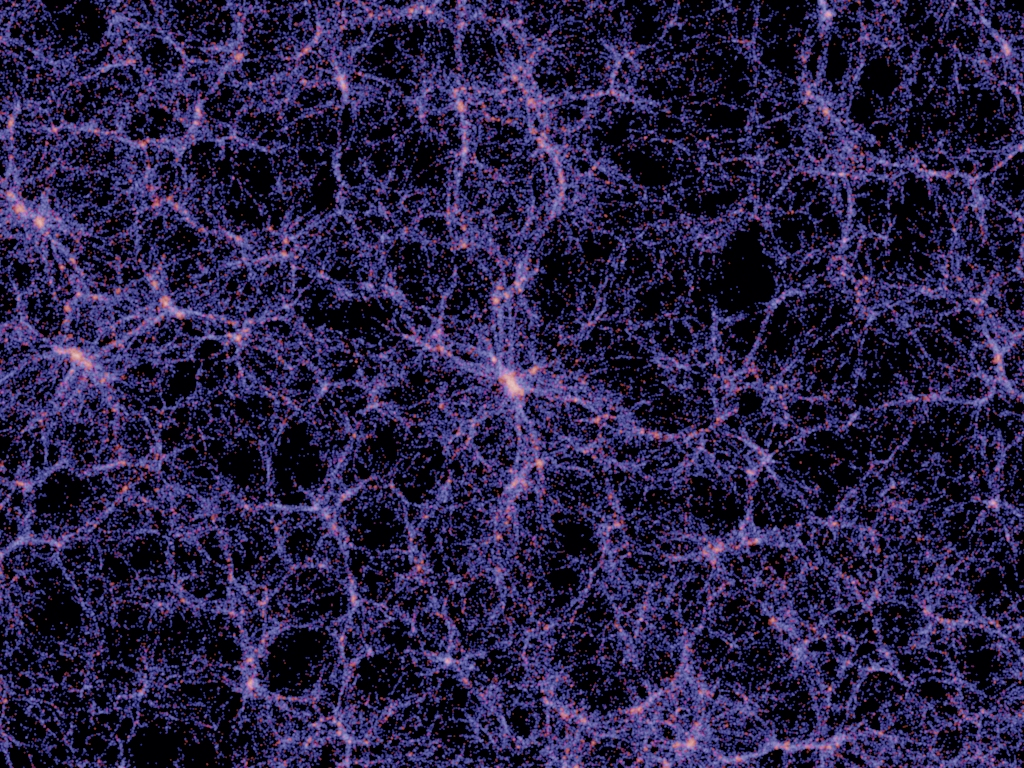
\includegraphics[width=0.95\textwidth]{pictures/millenium.jpg}
    \caption{Die Abbildung zeigt eine grafische Ausgabe der Milleniums-Simulation, welche versucht unser gesamtes Universum nachzustellen. Es wird deutlich, dass Galaxienhaufen auf großem Maßstab eine netzartigen Struktur bilden. Eine solche Aussage hätte man unmöglich nur durch theoretische Berechnungen treffen können. \\ Quelle: \\ \milleniumurl}
    \label{fig:millenium}
  \end{figure}

% section einleitung (end)